\chapter{Google earth}\label{ap:GE}

Es posible utilizar el \href{https://www.google.com/earth/desktop/}{Google Earth Pro} como herramienta de GIS para analizar los resultados obtenidos(Figura \ref{fig:gearth}). Para ello es necesario exportar la vista como KMZ y luego abrirla en Google Earth.

\begin{figure}[h!]
    \centering
    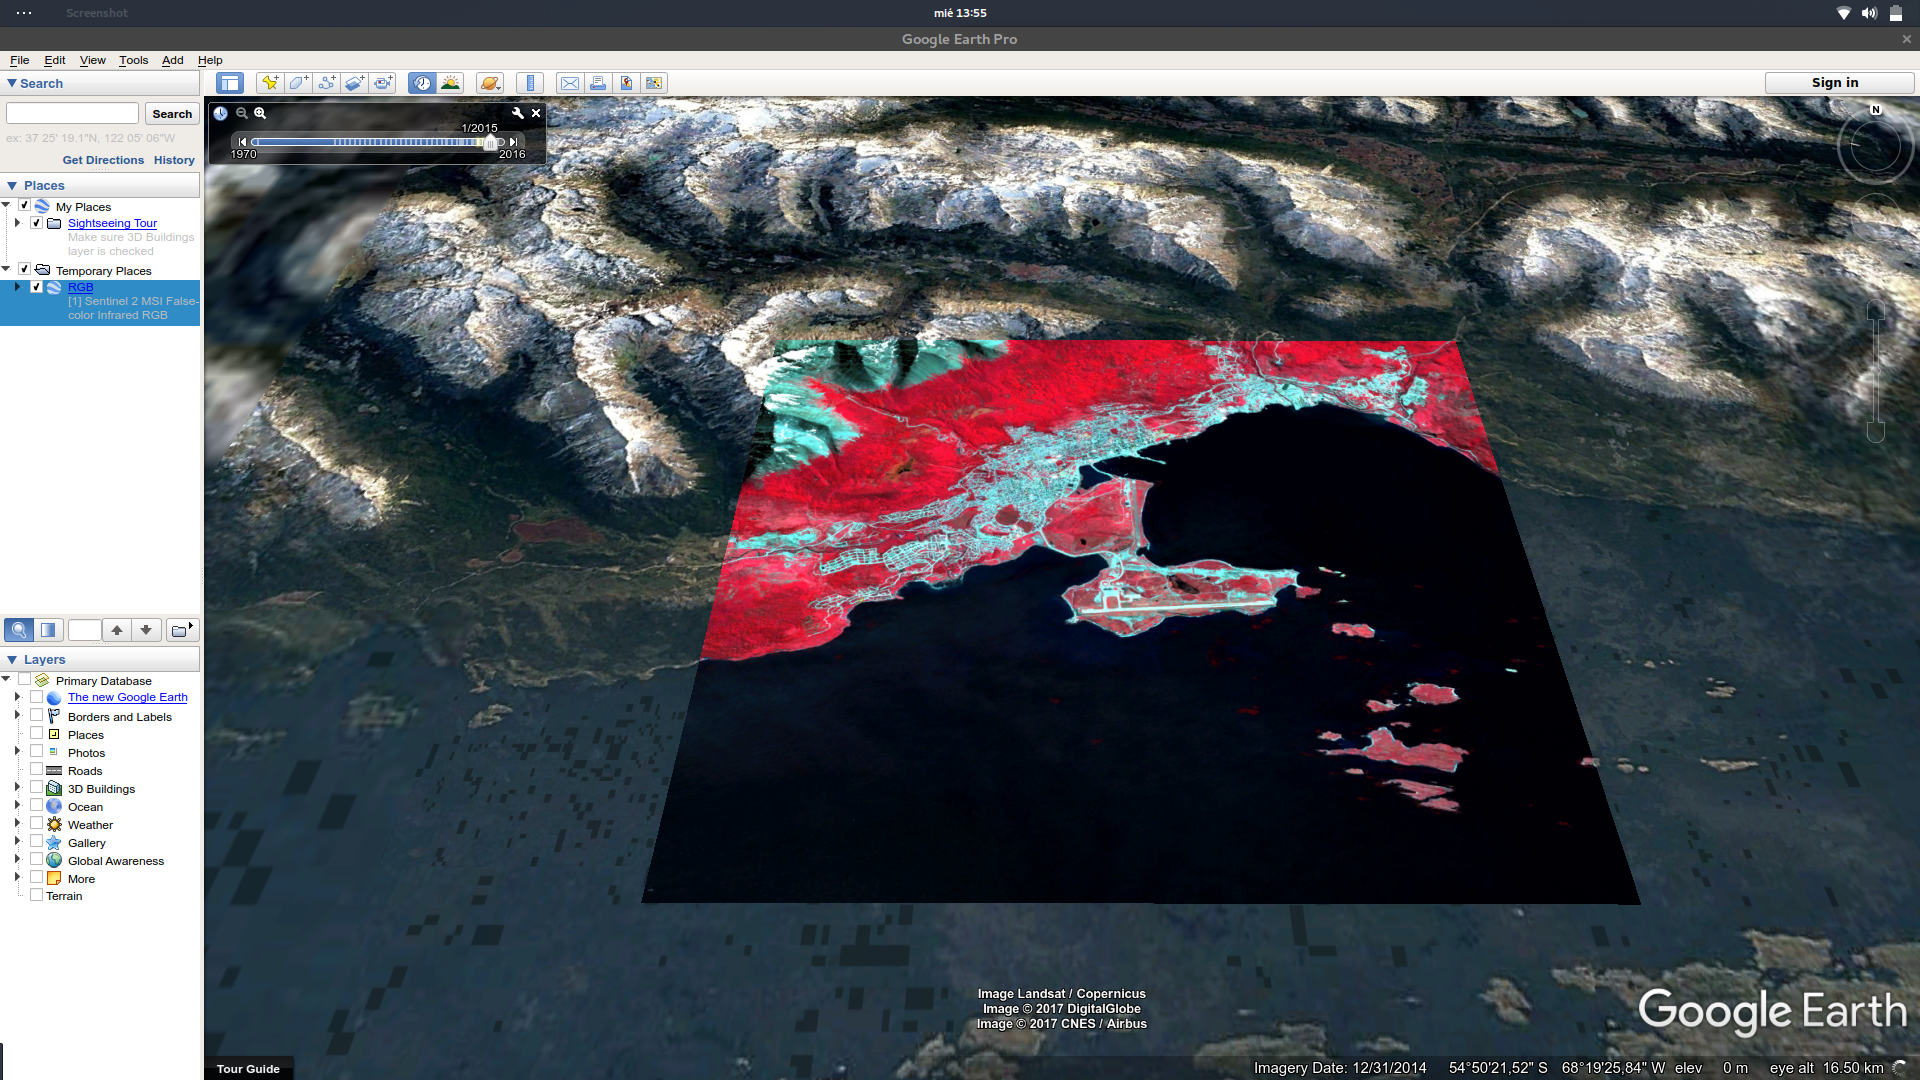
\includegraphics[width=0.7\textwidth]{fig:gearth.png}
    \caption{Imagen óptica de Ushuaia desplegada en Google Earth}
    \label{fig:gearth}
\end{figure}

\section{Creación de archivos KMZ}

Es posible exportar la visualización de la imagen completa o de una región específica desde \menu{File>Export view}. Si selecciona \menu{View as Google Earth KMZ} obtendrá un archivo \texttt{.kmz} que luego podrá abrir desde Google Earth.

Para realizar este proceso la imagen debe encontrarse proyectada en coordenadas geográficas (Apéndice \ref{ap:HA}) y solo se exportará la vista de la pantalla.

\section{Google Earth}

Al ejecutar Google Earth se encontrará con una vista del mundo. Para abrir un archivo \directory{.kmz} diríjase a \menu{File>Open...}. Seleccione el archivo que exporto del \emph{SNAP} y Google Earth se desplazará automáticamente hasta donde se encuentra el archivo (Figura \ref{fig:gearth}).

Es posible mostrar distintas coberturas seleccionándolas de la sección \menu{Places} a la derecha de la pantalla.
